\documentclass{standalone}

\usepackage{pgfplots}
\pgfplotsset{compat=1.12}

\begin{document}

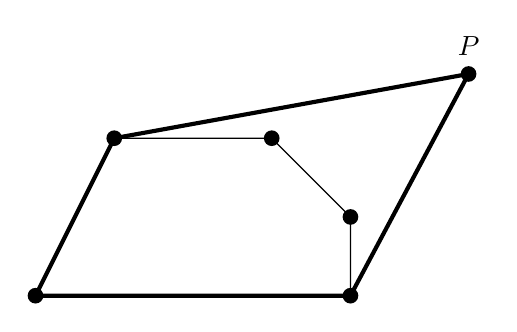
\begin{tikzpicture}
\draw[line width=0.5pt] (0.0, 0.0)
-- (4.0, 0.0)
-- (4.0, 1.0)
-- (3.0, 2.0)
-- (1.0, 2.0)
-- cycle;
\draw[line width=1.5pt] (0.0, 0.0)
-- (4.0, 0.0)
-- (5.5, 2.81596017514019)
-- (1.0, 2.0)
-- cycle;
\node [circle, fill=black, inner sep=2pt] at (0.00000000, 0.00000000) {};
\node [circle, fill=black, inner sep=2pt] at (4.00000000, 0.00000000) {};
\node [circle, fill=black, inner sep=2pt] at (4.00000000, 1.00000000) {};
\node [circle, fill=black, inner sep=2pt] at (3.00000000, 2.00000000) {};
\node [circle, fill=black, inner sep=2pt] at (1.00000000, 2.00000000) {};
\node [circle, fill=black, inner sep=2pt, label={above:$P$}] at (5.5, 2.81596017514019) {};
\end{tikzpicture}
\end{document}